\chapter{Introduction to the OPUS GUI}

This section of the documentation provides a tutorial approach to using the new The Graphical Interface (GUI) that has been added to the OPUS system as of version 4.2.  This represents a substantial initiative to make UrbanSim and OPUS more user-friendly and accessible to modelers and model users -- by reducing the need for programming expertise to use the system effectively to build, estimate, and use model systems for a range of applications.  We think the GUI offers a substantial advance in usability, and look forward to user feedback, and contributions from collaborators, to continue building on this foundation.

If you haven't already, please install Opus and UrbanSim on your machine.
Installation instructions are in Appendix~\ref{appendix:installation}.

\section{Main Features}

The GUI is cross-platform compatible, and has been developed using the open source Qt4 library.  
Note that screenshots included in this section will be taken from all three platforms, to give a 
sense of the look and feel of the GUI on each platform.  After launching the GUI from any of these platforms, 
the main Opus GUI window should be displayed as in Figure \ref{fig:opus1-linux} or \ref{fig:opus1-mac} . 

The organization of the GUI is based on an expectation that the work flow for developing and using models can be effectively organized into tasks that follow an ordering of data management, model management, scenario management, and results management.  The main window of the GUI reflects this work flow expectation, by implementing four tabs in the left-hand panel of the main window labeled \emph{Data Manager}, \emph{Model Manager}, \emph{Scenario Manager}, and \emph{Results Manager}.  Each tab provides a container for configuring and running a variety of tasks, organized into the main functional areas involved in developing and using a simulation model.  

\squishlist
\item The \emph{Data Manager} organizes the processes related to moving data between the Opus environment and, doing data processing both within Opus, and also remotely in a database or GIS environment.  Opus can use Python to pass data and commands to a database system like Postgres or MS SQL Server, or to a GIS system like ArcGIS or PostGIS.  Tasks can be organized in the Data Manager as scripts, and run as a batch, or alternatively, they may be run interactively.
\item The \emph{Model Manager} organizes the work of developing, configuring, and estimating the parameters of models, and of combining models into a model system.
\item The \emph{Scenario Manager} organizes the tasks related to configuring a scenario of input assumptions, and to interact with a run management system to actually run simulations on scenarios.  Tools to monitor and interact with a running simulation are provided here.
\item The \emph{Results Manager} provides the tools to explore results once one or more scenarios have been simulated.  It integrates an Indicator Framework that makes it possible to generate a variety of indicators, for diagnostic and for evaluation purposes.  It also provides functionality to visualize indicators as charts, maps, and tables, and to export results to other formats for use outside of Opus.
\squishend


To launch the Opus GUI, you will need to run a python script
called opus.py in the /opus/src/opus\_gui directory\footnote{Note the
use of forward slashes in the path.  On most operating systems, and in
Python, forward slashes are used to indicate separations in the path
components.  On Windows, backward slashes are used instead.  Python can
actually use forward slashes and translate them appropriately on
Windows or other operating systems as needed, so we will use the
convention of forward slashes throughout the text, for generality.}. 
If you have used the Windows installer to install Opus, then a Windows
\texttt{Start} menu item has been added under the Opus menu item
under programs, so launching Opus is a simple as selecting the
\texttt{OpusGUI Opus} menu item.  If you did not use the installer,
for example, on OS X, or Linux, then open a command window or shell, change directory to
the opus\_gui directory and type \texttt{python opus.py}.  In Windows,
you can also double-click on the opus.py file in the
/opus/src/opus\_gui directory to launch the GUI.\\

However it is launched, it will start from a command shell, and this
window remains active while Opus is running.  Do not attempt to quit
this window or Opus will close also.  


\begin{figure}[htp]
\begin{center}
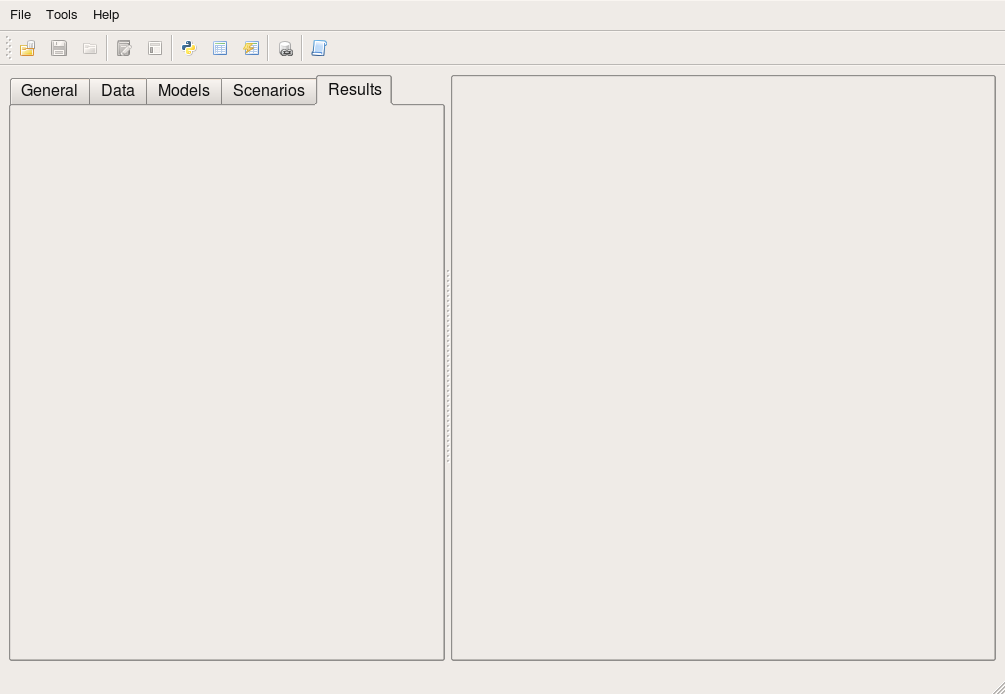
\includegraphics[scale=0.42]{part-gui/images/opus-startup.png}
\end{center}
\caption{Opus GUI Main Window - on Ubuntu Linux}
\label{fig:opus1-linux}
\end{figure}

\begin{figure}[htp]
\begin{center}
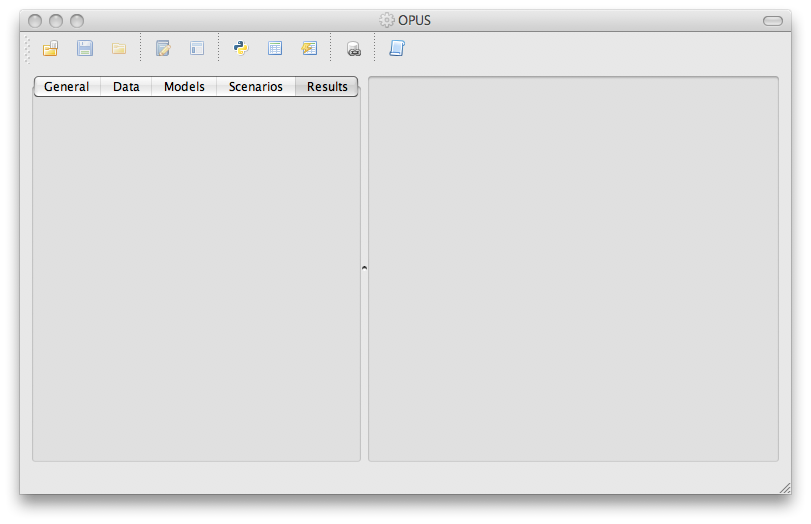
\includegraphics[scale=0.52]{part-gui/images/opus-startup-mac.png}
\end{center}
\caption{Opus GUI Main Window - on Leopard}
\label{fig:opus1-mac}
\end{figure}

